\subsection{AIME (American Invitational Mathematics Examination)}
{{\footnotesize
\noindent The AIME is a 15-question, 3-hour exam for high-school students featuring challenging
short-answer math problems in algebra, number theory, geometry, and combinatorics, 
assessing depth of problem-solving ability.


\begin{description}[labelwidth=4cm, labelsep=1em, leftmargin=4cm, itemsep=0.1em, parsep=0em]
  \item[date:] 2025-03-13
  \item[version:] 1
  \item[last\_updated:] 2025-03-13
  \item[expired:] false
  \item[valid:] yes
  \item[valid\_date:] 2025-03-13
  \item[url:] \href{https://artofproblemsolving.com/wiki/index.php/AIME\_Problems\_and\_Solutions}{https://artofproblemsolving.com/wiki/index.php/AIME\_Problems\_and\_Solutions}
  \item[doi:] NA
  \item[domain:] Mathematics
  \item[focus:] Pre-college advanced problem solving
  \item[keywords:]
    - algebra
    - combinatorics
    - number theory
    - geometry
  \item[licensing:] unknown
  \item[task\_types:]
    - Problem solving
  \item[ai\_capability\_measured:]
    - Mathematical problem-solving and reasoning
  \item[metrics:]
    - Accuracy
  \item[models:]
    - unkown
  \item[ml\_motif:]
    - Math problem solving
  \item[type:] Benchmark
  \item[ml\_task:]
    - Supervised Learning
  \item[solutions:] 0
  \item[notes:] Designed for human test-takers
  \item[contact.name:] unknown
  \item[contact.email:] unknown
  \item[datasets.links.name:] AoPS website
  \item[datasets.links.url:] \href{https://artofproblemsolving.com/wiki/index.php/AIME\_Problems\_and\_Solutions}{https://artofproblemsolving.com/wiki/index.php/AIME\_Problems\_and\_Solutions}
  \item[results.links.name:] unknown
  \item[results.links.url:] \href{unknown}{unknown}
  \item[fair.reproducible:] True
  \item[fair.benchmark\_ready:] True
  \item[id:] aime\_american\_invitational\_mathematics\_examination
  \item[Citations:] \cite{www-aime}
\end{description}

{\bf Ratings:} ~ \\

\begin{tabular}{p{0.15\textwidth} p{0.07\textwidth} p{0.7\textwidth}}
\hline
Rating & Value & Reason \\
\hline
dataset & 4 & Easily accessible data with problems and solutions, but no splits
 \\
documentation & 0 & Not given
 \\
metrics & 5 & (by default) Answer is correct or it's not
 \\
reference\_solution & 0 & Not given. Human performance stats exist, but no mentions of AI performance
 \\
software & 0 & No code available
 \\
specification & 0 & Obvious what the problems are, but not specified how to administer them to AI models. No HW constraints
 \\
\hline
\end{tabular}

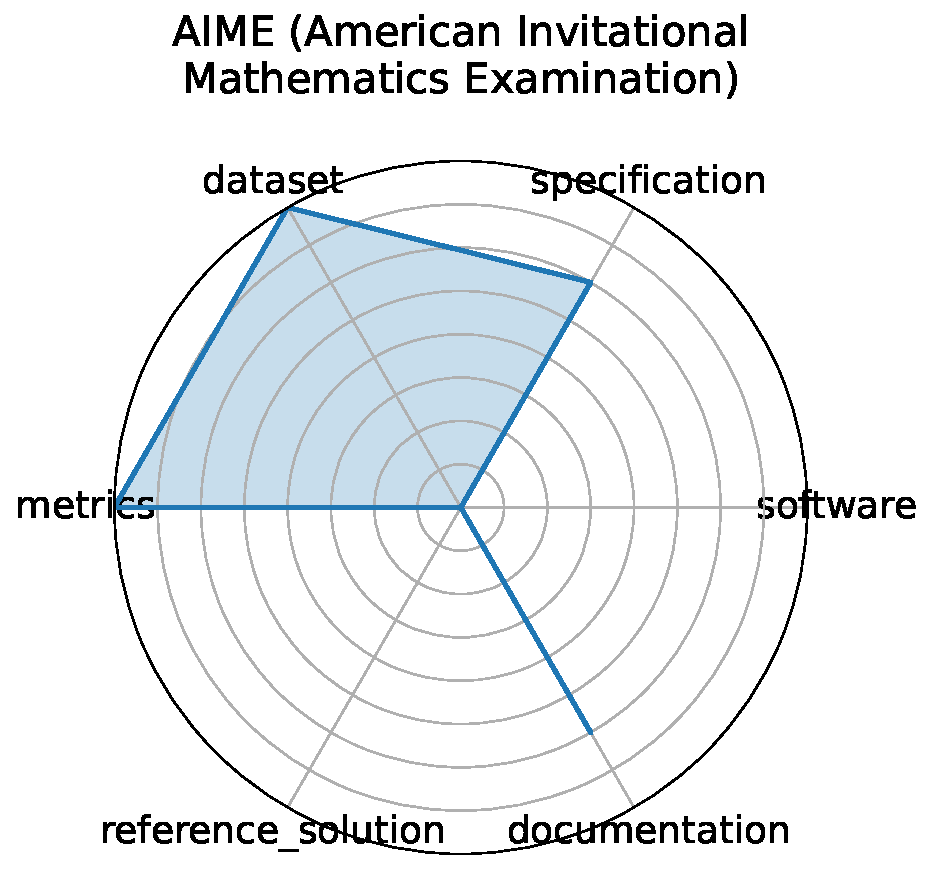
\includegraphics[width=0.2\textwidth]{aime_american_invitational_mathematics_examination_radar.pdf}
}}
\clearpage